\chapter{Background}

The basis for this continued work stems from multi-dimensional data structures
and how they are leveraged in a geospatial environment. These data structures,
the Quadtree, Octree, and K-D Tree, are used to partition a (usually) Cartesian
coordinate system into a tree structure.

\section{Quadtree}

The Quadtree separates a two-dimensional coordinate system into a tree structure
where each node in the tree is split along the center of both axes within its
axis-aligned bounding volume creating four child nodes. This allows for much
more efficient searching than a simple data structure like an array or list
would. Below, \ref{fig:quadtree} shows a set of points in a two-dimensional
Cartesian coordinate system stored in a Quadtree where each node that has only a
single point remaining does not split again; thus saving computational time and
storage space. The Quadtree structure is used in geospatial visualizations as it
aligns to the longitude and latitude coordinate system, however, the disconnect
along the 180-degree meridian and the difficult-to-handle north and south border
meeting at a single point cause more issues.

\begin{figure}[htb]
\begin{center}
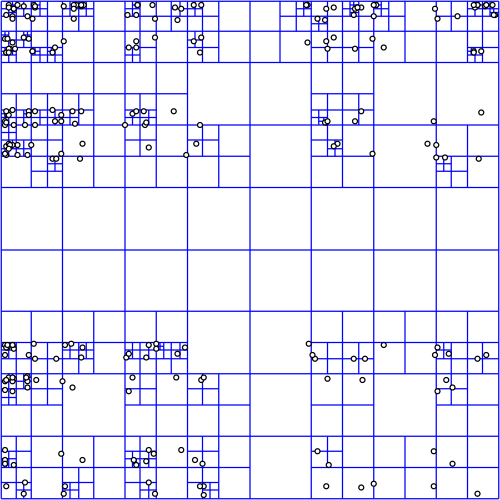
\includegraphics[width=.5\linewidth]{images/Point_quadtree.png}
\end{center}
\caption{Quadtree Structure {\cite{10_eppstein_2005}}}
\label{fig:quadtree}
\end{figure}

\section{Octree}

The Octree structure is identical to the Quadtree structure except that it is
applied to a three-dimensional coordinate system. Each node is split into
potentially eight child nodes but it still uses a uniform split location by
bisecting the span along each axis of its axis-aligned bounding volume. The
Octree is used quite often in Computer Graphics as it fits well to an XYZ
Cartesian coordinate system and allows culling, bounds intersection, and mouse
picking for many objects quickly and efficiently. However, in a geospatial
visualization, this structure does not align well to an elliptical surface such
as the Earth. Below, \ref{fig:octree} is an image of an Octree in 3D as well as the
flattened version of the tree.

\begin{figure}[htb]
\begin{center}
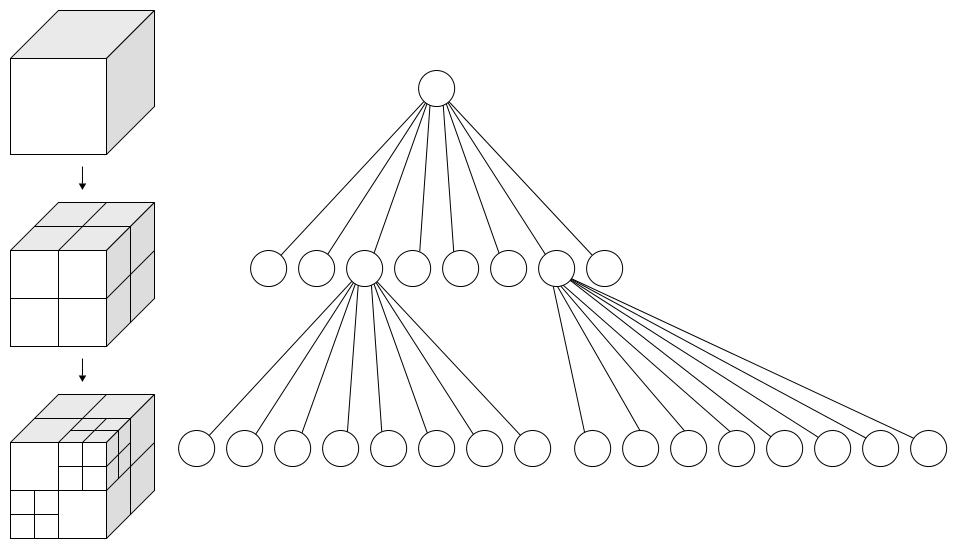
\includegraphics[width=.9\linewidth]{images/Octree_flat.png}
\end{center}
\caption{Octree Structure and Flattened Tree \cite{11_octree2.png}}
\label{fig:octree}
\end{figure}

\section{k-d tree}

The K-D Tree is a specialized binary tree that allows for more control over how
the tree is structured as well as lending itself to being more uniform and
balanced than previously mentioned tree data structures. The K-D Tree, at each
level, chooses a single axis to split along. The axis chosen is defined by a set
of criteria such as which axis has the longest span between its min and max
values. Then, the split location is also defined by a set of criteria such as
splitting each side into containing a uniform number of points. The actual split
location, unlike the Quadtree and Octree, is a single point that acts as the
node in the tree at that depth. This continues until each node has a single
point or until some threshold is reached based on tree depth or point count. The
K-D Tree is a binary tree but can be used with any dimensionality which allows
it to be applied to a two-dimensional longitude-latitude coordinate system as
with the Quadtree and an XYZ Cartesian coordinate system like the Octree. It has
many of the same drawbacks when it comes to applying it to a geospatial
coordinate system. However, one upside is that it can be built in such a way
that each node has a relatively uniform number of points which can increase
storage efficiency and render times by allowing the storage of nodes in chunks
without wasting padded space but with the drawback that level-of-detail
algorithms make the scene seem non-uniform as each node is rendered and the node
dimensions are not consistent. Below, \ref{fig:kdtree2d} shows a two-dimensional K-D Tree
partitioning algorithm with red and blue lines as alternating split locations.
\ref{fig:kdtreelayers} shows the flattened tree structure for part of the previous figure and
which axis was used at each level.

\begin{figure}[htb]
\begin{center}
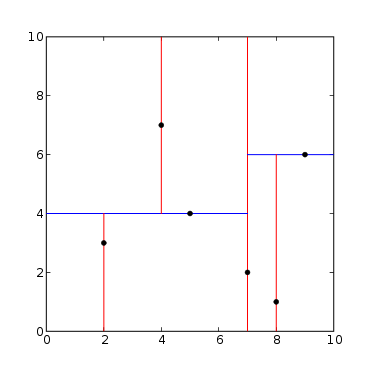
\includegraphics[width=.5\linewidth]{images/kdtree_2d.png}
\end{center}
\caption{Two-Dimensional K-D Tree Structure \cite{12_kdtree_2d.svg}}
\label{fig:kdtree2d}
\end{figure}

\begin{figure}[htb]
\begin{center}
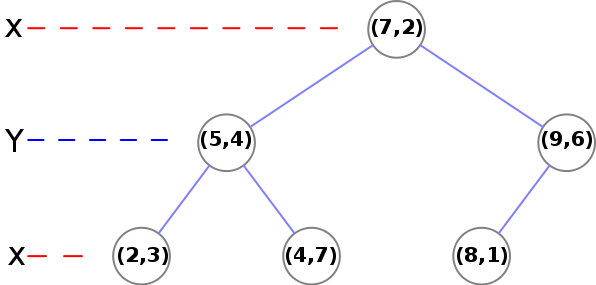
\includegraphics[width=.5\linewidth]{images/kdtree_layers.png}
\end{center}
\caption{K-D Tree Partitioning Example \cite{13_tree_0001.svg}}
\label{fig:kdtreelayers}
\end{figure}

Previously, Quadtree, Octree \cite{3_wenzel2014out} and K-D Tree partitioning
systems have been applied to a Cartesian system in order to add on-demand
searching for view-dependent slices of data. However, once the data set is
converted into a geospatial positioning system, either the Cartesian coordinates
are now not surface aligned, or issues arise along the partitioning system
boundaries where values are not continuous (such as with latitude 90 != latitude
-90 but longitude 180 == longitude -180). Using a Cartesian projection from
geospatial coordinates solves this issue but adds complexity when deciding what
to render as it is no longer surface aligned. This paper looks into applying a
surface-aligned data structure to a global data set such as a tetrahedral mesh.
By using this structure to search for nodes within the view frustum the
visualization system will be able to render progressively deeper nodes as the
visualization's viewpoint moves closer or further away from the target and as
the level of detail increases and will then pull these nodes from an on-demand
point server or local file system cache.

Also, in recent work, real-time rendering of depth culling and surface
representation \cite{1_VAST:VAST11:105-112} has been used to hide unseen data
points as well as to fill surface information in on a massive unstructured point
cloud. This paper proposes to use this information and apply it to a sparse
context-aware selection algorithm \cite{2_yu:hal-01178051} in order to adapt it
to a more uniformly dense data set. This on-the-fly surface creation can be used
to augment the context-aware selection algorithm in order to give it another
avenue for object separation qwithin a uniformly-dense data set.
